\documentclass[journal]{vgtc}                % final (journal style)
%\documentclass[review,journal]{vgtc}         % review (journal style)
%\documentclass[widereview]{vgtc}             % wide-spaced review
%\documentclass[preprint,journal]{vgtc}       % preprint (journal style)

%% Uncomment one of the lines above depending on where your paper is
%% in the conference process. ``review'' and ``widereview'' are for review
%% submission, ``preprint'' is for pre-publication, and the final version
%% doesn't use a specific qualifier.

%% Please use one of the ``review'' options in combination with the
%% assigned online id (see below) ONLY if your paper uses a double blind
%% review process. Some conferences, like IEEE Vis and InfoVis, have NOT
%% in the past.

%% Please note that the use of figures other than the optional teaser is not permitted on the first page
%% of the journal version.  Figures should begin on the second page and be
%% in CMYK or Grey scale format, otherwise, colour shifting may occur
%% during the printing process.  Papers submitted with figures other than the optional teaser on the
%% first page will be refused. Also, the teaser figure should only have the
%% width of the abstract as the template enforces it.

%% These few lines make a distinction between latex and pdflatex calls and they
%% bring in essential packages for graphics and font handling.
%% Note that due to the \DeclareGraphicsExtensions{} call it is no longer necessary
%% to provide the the path and extension of a graphics file:
%% 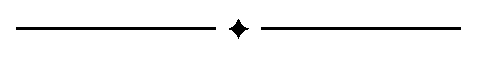
\includegraphics{diamondrule} is completely sufficient.
%%
\ifpdf%                                % if we use pdflatex
  \pdfoutput=1\relax                   % create PDFs from pdfLaTeX
  \pdfcompresslevel=9                  % PDF Compression
  \pdfoptionpdfminorversion=7          % create PDF 1.7
  \ExecuteOptions{pdftex}
  \usepackage{graphicx}                % allow us to embed graphics files
  \DeclareGraphicsExtensions{.pdf,.png,.jpg,.jpeg} % for pdflatex we expect .pdf, .png, or .jpg files
\else%                                 % else we use pure latex
  \ExecuteOptions{dvips}
  \usepackage{graphicx}                % allow us to embed graphics files
  \DeclareGraphicsExtensions{.eps}     % for pure latex we expect eps files
\fi%

%% it is recomended to use ``\autoref{sec:bla}'' instead of ``Fig.~\ref{sec:bla}''
\graphicspath{{figures/}{pictures/}{images/}{./}} % where to search for the images

\usepackage{microtype}                 % use micro-typography (slightly more compact, better to read)
\PassOptionsToPackage{warn}{textcomp}  % to address font issues with \textrightarrow
\usepackage{textcomp}                  % use better special symbols
\usepackage{mathptmx}                  % use matching math font
\usepackage{times}                     % we use Times as the main font
\renewcommand*\ttdefault{txtt}         % a nicer typewriter font
\usepackage{cite}                      % needed to automatically sort the references
\usepackage{tabu}                      % only used for the table example
\usepackage{booktabs}                  % only used for the table example
%% We encourage the use of mathptmx for consistent usage of times font
%% throughout the proceedings. However, if you encounter conflicts
%% with other math-related packages, you may want to disable it.

%% In preprint mode you may define your own headline.
%\preprinttext{To appear in IEEE Transactions on Visualization and Computer Graphics.}

%% If you are submitting a paper to a conference for review with a double
%% blind reviewing process, please replace the value ``0'' below with your
%% OnlineID. Otherwise, you may safely leave it at ``0''.
\onlineid{0}

%% declare the category of your paper, only shown in review mode
\vgtccategory{Research}
%% please declare the paper type of your paper to help reviewers, only shown in review mode
%% choices:
%% * algorithm/technique
%% * application/design study
%% * evaluation
%% * system
%% * theory/model
\vgtcpapertype{algorithm/technique}

%% Paper title.
\title{Project 02 Proposal: WhatAreWeDoingQuestionMark}

%% This is how authors are specified in the journal style

%% indicate IEEE Member or Student Member in form indicated below
\author{Emmitt R Johnson, Makiah Merritt, and David Shingai Ntuli}
\authorfooter{
    %% insert punctuation at end of each item
    \item
    Emmitt R Johnson. E-mail: johnemmi@oregonstate.edu.
    \item
    Makiah Merritt. E-mail: merrittm@oregonstate.edu.
    \item
    David Shingai Ntuli. E-mail: ntulid@oregonstate.edu.
}


%other entries to be set up for journal
\shortauthortitle{Biv \MakeLowercase{\textit{et al.}}: DontKnowWhatWeAreDoing}
%\shortauthortitle{Firstauthor \MakeLowercase{\textit{et al.}}: Paper Title}

%% Abstract section.
\abstract{
    The projects that looks interesting to us were \textit{VisDock}, \textit{HindSight}, and \textit{PROACT}, and they all brought something a bit different to the table. We looked at several other papers, but there were various challenges that would make them difficult to pursue. 
} % end of abstract

%% Keywords that describe your work. Will show as 'Index Terms' in journal
%% please capitalize first letter and insert punctuation after last keyword
\keywords{}

%% ACM Computing Classification System (CCS).
%% See <http://www.acm.org/class/1998/> for details.
%% The ``\CCScat'' command takes four arguments.

\CCScatlist{ % not used in journal version
    \CCScat{K.6.1}{Management of Computing and Information Systems}%
    {Project and People Management}{Life Cycle};
    \CCScat{K.7.m}{The Computing Profession}{Miscellaneous}{Ethics}
}

%% Uncomment below to include a teaser figure.
% \teaser{
%     \centering
%     \includegraphics[width=\linewidth]{CypressView}
%     \caption{In the Clouds: Vancouver from Cypress Mountain. Note that the teaser may not be wider than the abstract block.}
%     \label{fig:teaser}
% }

%% Uncomment below to disable the manuscript note
\renewcommand{\manuscriptnotetxt}{}

%% Copyright space is enabled by default as required by guidelines.
%% It is disabled by the 'review' option or via the following command:
\nocopyrightspace

\vgtcinsertpkg

%%%%%%%%%%%%%%%%%%%%%%%%%%%%%%%%%%%%%%%%%%%%%%%%%%%%%%%%%%%%%%%%
%%%%%%%%%%%%%%%%%%%%%% START OF THE PAPER %%%%%%%%%%%%%%%%%%%%%%
%%%%%%%%%%%%%%%%%%%%%%%%%%%%%%%%%%%%%%%%%%%%%%%%%%%%%%%%%%%%%%%%%

\begin{document}

%% The ``\maketitle'' command must be the first command after the
%% ``\begin{document}'' command. It prepares and prints the title block.

%% the only exception to this rule is the \firstsection command
% \firstsection{Introduction}

\maketitle

%% \section{Introduction} %for journal use above \firstsection{..} instead
% \textbf{Do we need an intro?} Lorem ipsum dolor sit amet, consetetur sadipscing elitr, sed diam nonumy eirmod tempor invidunt ut labore et dolore magna aliquyam erat, sed diam voluptua.

% Instructions:
% for each paper
%   (1) write a paragraph explaining the paper (problem statement, technique, results). Be sure to paraphrase instead of copying/pasting the abstract or other parts of the papers.
%   (2) write a paragraph explaining how this paper may relate to your term project (a better technique, a novel application of the same technique, etc). Furthermore, list the challenges if you were to work on this paper.

\section{Related Papers}
    \subsection{Paper 01: \textit{VisDock: A Toolkit for Cross-Cutting Interactions in Visualization} \cite{VisDock:2014}}
        \subsubsection{Paper Description}
        Prepared by Jungu Choi, Deok Gun Park, Yuet Ling Wong, Eli Fisher, and Niklas Elmqvist, Senior Member, IEEE; this paper reviews a tool the team created to provide ``a core set of cross-cutting interaction techniques for visualization'' \cite[p.~1]{VisDock:2014}.
        The tool, VisDock, was created as a plugin library using JavaScript to interact with visualizations based on SVGs; upon completion of the tool, the team released it as Open Source.
        A qualitative study with four developers and 11 end-users ``found the tool usable and efficient'' \cite[p.~2]{VisDock:2014}.

        \subsubsection{Project Value}
        In their future work section, one area of interest is the implementation of data-level interactions for ``filtering, searching, and drilling down into the data'' \cite[p.~12]{VisDock:2014}. Along these lines we could investigate ways to provide interactions allowing quick manipulations of the graph based upon data selections of the user. For example, supposing the user would like to find similar elements in the data set based upon a selection, we could look into developing a way to generate visual changes to make those elements stand out. Problems we may encounter mainly surround picking up and applying the VisDock. Although documentation and examples will be available, being open source there is no guarantee that it will be plug and play. Furthermore, the implementation of VisDock is that of a plug-in, meaning we will need to start the visualization another visualization tool such as D3 and figure out the extent of VisDock's manipulation capabilities.

        In their future work section, one area of interest is the implementation of data-level interactions for ``filtering, searching, and drilling down into the data'' \cite[p.~12]{VisDock:2014}.
        Along these lines we could investigate ways to provide interactions allowing quick manipulations of the graph based upon data selections of the user.
        For example, supposing the user would like to find similar elements in the data set based upon a selection, we could look into developing a way to generate visual changes to make those elements stand out.
        Problems we may encounter mainly surround picking up and applying the VisDock.
        Although documentation and examples will be available, being open source there is no guarantee that it will be plug and play.
        Furthermore, the implementation of VisDock is that of a plug-in, meaning we will need to start the visualization another visualization tool such as D3 and figure out the extent of VisDock's manipulation capabilities.

    \subsection{Paper 02: \textit{HindSight: Encouraging Exploration through Direct Encoding of Personal Interaction History} \cite{HindSight:2016}}
        \subsubsection{Paper Description}
        In this paper, HindSight is a term used to denote the technique where a user's interaction history with a data visualization is visually encoded \cite[p.~1]{HindSight:2016}.
        The authors, Mi Feng, Cheng Deng, Evan M. Peck, and Lane Harrison, studied how HindSight designs impact user exploration and interaction with a visualization.
        HindSight principles are designed to ease the burden on a user's short-term memory, as exploration of data visualizations are limited by a user's ability to remember recent interactions.
        To examine the impact of HindSight designs, the researchers conducted studies using three different visualizations.
        Four hundred participants were tasked to explore a visualization, some of which had HindSight applied.
        The studies found that visualizations with HindSight applied appeared to allow users to explore more and different parts of the data.

        \subsubsection{Project Value}
        The purpose of this paper was to show how a simple low-barrier technique like HindSight might be able to change a user's exploration behavior.
        Possible work we could cover for a project includes examining how active design properties might benefit from passive design properties and vice versa.
        For instance, how bookmarking might benefit from HindSight.
        Another avenue for project work includes how more a more detailed history might be beneficial or detrimental when taking into account implementation complexity.
        Some challenges might include finding sources of data visualization that are openly available to us.


    \subsection{Paper 03: \textit{PROACT: Iterative Design of a Patient-Centered Visualization for Effective Prostate Cancer Health Risk Communication} \cite{PROACT:2016}}
        \subsubsection{Paper Description}
        PROACT (PROgnosis Assessment for Conservative Treatment) is a tool created and tested by Anzu Hakone, Lane Harrison, Alvitta Ottley, Nathan Winters, Caitlin Gutheil, Paul K. J. Han, Remco Chang to communicate risk information to individuals suffering from prostate cancer.
        ``PROACT utilizes two published clinical prediction models to communicate the patients’ personalized risk estimates and compare treatment options'' \cite[p.~1]{PROACT:2016}.
        With a primary goal of transmitting information across to emotionally charged individuals, the tool's design is backed by user studies of prostate cancer survivors and urologists from the Maine Medical Center.
        Through their study, they found an appropriate design required a easy to read bits of information that could likewise be easily comprehended with little effort.
        Specifically, listed in their \textit{findings} section, the team found a \textbf{temporal visualization} with \textbf{narrative sequence} worked best to communicate with varying \textbf{emotional state}s \cite[p.~8]{PROACT:2016}.
        This led the initial designs to use simple visualizations, such as pie and bar charts, minimal labeling, and present the data in a positive lens; noting ``adding interactions to either simple or complex visualizations had an adverse effect'' \cite[p.~2]{PROACT:2016}.

        \subsubsection{Project Value}
        As the team mainly focused on getting a narrative visualization in place, they left room to expand upon information communicated.
        Noted in their \textit{future work} section, adding other factors - ``side effects, recovery time, quality of life, localized vs. metastatic (cancer spread outside of the prostate), and other treatment options'' \cite[p.~9]{PROACT:2016} would be of great use in taking the next step, transitioning the tool from proof of concept.
        The team also desired the exploration of conveying quantified uncertainties in the clinical prediction models (CPMs).
        As we don't have easy access to this data, our primary desire would be the investigation of methods by which we could communicate the other factors impacting a patients decision on treatment plans.
        On such idea would be the application of a heat map to bodily area's that may be impacted by various treatments; where the hot spots would indicate a high likely hood for side effects.
        However, this is just one example.
        There are many other ways to communicate information; our goal in pursing this project would be to keep the teams original design considerations in mind.

\section{Referenced Papers}
    \begin{enumerate}
        \item{\textit{Vega-Lite: A Grammar of Interactive Graphics} (2016), Arvind Satyanarayan, Dominik Moritz, Kanit Wongsuphasawat, and Jeffrey Heer \cite{VegaLite:2016}}
        \item{\textit{Embedded Data Representations:2016} (2016), Wesley Willett, Yvonne Jansen, Pierre Dragicevic \cite{EmbeddedDataRepresentations:2016}}
        \item{\textit{The Attraction Effect in Information Visualization} (2016), Evanthia Dimara, Anastasia Bezerianos, and Pierre Dragicevic \cite{AttractionEffect:2016}}
        \item{\textit{Immersive Collaborative Analysis of Network Connectivity: CAVE-style or Head-Mounted Display?} (2016), Maxime Cordeil{,} Tim Dwyer{,} Karsten Klein{,} Bireswar Laha{,} Kim Marriott{,} and Bruce H. Thomas \cite{NetworkConnectivityAnalysis:2016}}
        \item{\textit{A Study of Layout, Rendering, and Interaction Methods for Immersive Graph Visualization} (2016), Oh-Hyun Kwon{,} Chris Muelder{,} Kyungwon Lee{,} and Kwan-Liu Ma \cite{ImmersiveGraphVisualization:2016}}
        \item{\textit{Small Multiples with Gaps} (2016), Meulemans{,} W.{,} Dykes{,} J.{,} Slingsby{,} A.{,} Turkay{,} C. and Wood{,} J. \cite{SmallMultiples:2016}}
        \item{\textit{CUBu: Universal real-time bundling for large graphs.} (2016), Matthew van der Zwan{,} Valeriu Codreanu{,} and Alexandru Telea \cite{CUBu:2016}}
    \end{enumerate}



% if specified like this the section will be committed in review mode
\acknowledgments{
    The authors wish to thank the authors of the referenced papers for their work upon which we will attempt to expand upon.
}

\nocite{*}
%\bibliographystyle{abbrv}
%\bibliographystyle{abbrv-doi}
%\bibliographystyle{abbrv-doi-narrow}
\bibliographystyle{abbrv-doi-hyperref}
%\bibliographystyle{abbrv-doi-hyperref-narrow}

\bibliography{references}
\end{document}
